\documentclass{beamer}
\usepackage[utf8]{inputenc}
\usepackage[T1]{fontenc}
\usepackage[bulgarian]{babel}
\usepackage{alltt}

\useoutertheme{shadow}
\setbeamercolor{title}{fg=red!80!black}
\usetheme[secheader]{Madrid}
\usecolortheme{crane}

%Тема 11.
%7.2 Constraints on Attributes and Tuples
%• Not-Null Constraints
%• Attribute-Based CHECK Constraints
%• Tuple-Based CHECK Constraints
%• Modification of Constraints
%• Giving Names to Constraints
%• Altering Constraints on Tables

\title[Дървовидни структури за многомерни данни в MySQL]{Дървовидни структури за многомерни данни в MySQL}
\author{Валентина Динкова, ф.н. 71112}
\institute{ФМИ}
\date{\today}
\begin{document}
\begin{frame}
  \titlepage
\end{frame}
%\begin{frame}
  %\frametitle{Съдържание}
  %\tableofcontents
%\end{frame}

\begin{frame}
  \frametitle{GIS и разширението на MySQL за пространствени данни}
\begin{itemize}
 \item Какво е \textbf{GIS} и какво е \textbf{OGC}?
\end{itemize}
\textbf{GIS} означава Географска Информационна Система и е един от най-очевидните примери за пространствени данни.
\newline
\newline
\textbf{OGC} е организация, която работи по стандартизирането на различни области на GIS.
Един такъв стандарт е и спецификацията за SQL, която определя разширение на SQL базирани релационни бази данни, което да използва GIS обекти и операции.
\end{frame}

\begin{frame}
 OGC работи в 4 важни области:
\begin{itemize}
 \item типове данни;
 \item операции;
 \item възможност да се подават като вход и да се извеждат GIS данни;
 \item индексиране на пространствени данни.
\end{itemize}
Друга важна област са метаданните
\end{frame}
%  \begin{alltt}
%CREATE TABLE Person (
%    address VARCHAR(255) \alert{NOT NULL}
%);
%   \end{alltt}

\begin{frame}
\frametitle{Стандартът, използван от почти всички SQL бази данни с пространствено разширение, включително и MySQL}
\begin{center}
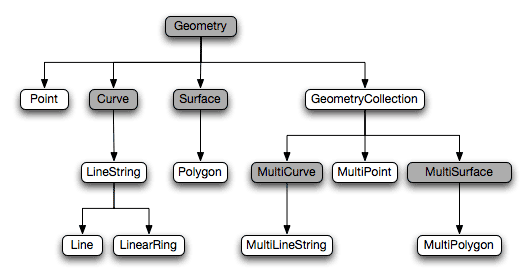
\includegraphics[width=60mm]{gis-datatypes.png}\end{center}
Типовете, отбелязани в сиво са абстракти и обекти от тези типове не могат да се създават.
\end{frame}

\begin{frame}
 \frametitle{Пространствени индекси}
\end{frame}


\end{document}